\documentclass[10pt, aspectratio=169]{beamer}

\usetheme[progressbar=frametitle]{metropolis}
\usepackage{appendixnumberbeamer}

\usepackage{booktabs}
\usepackage[scale=2]{ccicons}

\usepackage{pgfplots}
\usepgfplotslibrary{dateplot}
\definecolor{customgrey}{RGB}{240,240,240} % Light grey
\definecolor{customorange}{RGB}{255,102,0} % Orange
\usepackage[most]{tcolorbox}
\usepackage{lmodern}
\usepackage{listings}
\usepackage{xcolor}
\usepackage{amsmath}
\usepackage{animate}
\usepackage{svg}
\usepackage{threeparttable}
\usepackage{csquotes}
\usepackage{multicol}
\usepackage[dvipsnames]{xcolor}

\definecolor{CompBlue}{HTML}{1f77b4}
\definecolor{CompGreen}{HTML}{4daf4a}
\definecolor{CompRed}{HTML}{e41a1c}

\usepackage[
    backend=biber, 
    style=apa,
    hyperref=true
    ]{biblatex}
\addbibresource{latex/references.bib}

\definecolor{lightgray}{gray}{0.95}

%%% COLOR FOR EQUATIONS
\definecolor{myorange}{HTML}{FF7F0E}
\definecolor{myblue}{HTML}{984EA3}
\newtcblisting{promptblock}{
  colback=lightgray,
  colframe=,
  listing only,
  listing options={
    basicstyle=\ttfamily\small,
    breaklines=true,
    columns=fullflexible,
    keepspaces=true
  },
  title=,
  fonttitle=\bfseries,
  enhanced,
  boxrule=0.8pt,
  sharp corners,
  left=2mm,
  right=2mm,
  top=1mm,
  bottom=1mm
}
\setbeamercolor{block title alerted}{fg=white,bg=customorange}
\setbeamercolor{block body alerted}{fg=black,bg=customgrey}
\setbeamerfont{block title alerted}{series=\bfseries}
\setbeamerfont{block body alerted}{}
\usepackage{xspace}
\newcommand{\themename}{\textbf{\textsc{metropolis}}\xspace}


\title{Folk Around and Find Out}
\subtitle{Algorithmic Collusion and the Limits of Coordination}

% \date{\today}
\date{}
\author{Lucia Sauer, Julián Romero \& Moritz Peist}
\institute{Barcelona School of Economics}
%\logo{\includesvg[width=0.2\linewidth]{latex/imgs/BSE Barcelona Graduate School of Economics.svg}}
% \titlegraphic{\hfill\includegraphics[height=1.5cm]{logo.pdf}}

\begin{document}

\maketitle

\begin{frame}{Outline}
    \begin{columns}[c]
        \begin{column}{0.45\textwidth}
            \tableofcontents
        \end{column}
        \begin{column}{0.45\textwidth}
            \begin{figure}
                \centering
                \animategraphics[controls, 
                    autoplay, % Starts playing immediately
                    autoresume, % Resumes after page focus returns
                    autopause, % Pauses when page loses focus
                    poster=last, % picture to display when not playing
                    loop, % Loop through animation endlessly
                    width=0.7\linewidth]{20}{latex/slides_pricing_collusion/imgs/fafo/frame_}{00}{98}
                \caption{Will we find out?}
                \label{fig:fafo}
            \end{figure}
        \end{column}
    \end{columns}
\end{frame}

%%%%%%%%%%%%%%%%%%%%%%%%%%%%%%%%%%%%%%%%%%%%%%%%%%%%%%%%%%%%%%%%%%%%%%%%%%%%%%%%%%%%%%%%%%%%%%%%%%%%%%

\section{Introduction}

\begin{frame}{Motivation}
\begin{figure}
        \centering
        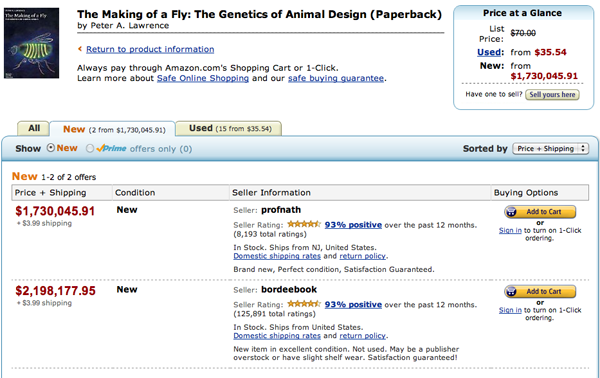
\includegraphics[width=0.65\linewidth]{latex/slides_pricing_collusion/imgs/the_making_of_a_fly.png}
        \caption{Two pricing algorithms made a biology textbook cost \$23 million. As Margrethe Vestager \parencite*{vestager_algorithms_2017} put it: \enquote{\emph{someone finally noticed $\ldots$ and adjusted it manually.}}}
        \label{fig:rep_org}
    \end{figure}  
\end{frame}

\begin{frame}{Theoretical Foundations: Algorithmic Collusion}
    \begin{columns}[c]
    \column{0.48\textwidth}
    \begin{block}{\textbf{\textcite{calvano_artificial_2020}: Foundational Theory}}
    \begin{itemize}
        \item \textbf{Method:} Q-learning algorithms in simulated Bertrand competition
        \item \textbf{Key Finding:} Algorithms autonomously learn to collude without explicit instructions
        \item \textbf{Mechanism:} Trial-and-error learning discovers punishment schemes
        \item \textbf{Implication:} Collusion possible without communication or agreement
    \end{itemize}
    \end{block}
    
    \column{0.48\textwidth}
    \begin{block}{\textbf{\textcite{fish_algorithmic_2025}: Modern AI Capabilities}}
    \begin{itemize}
        \item \textbf{Method:} LLM-based pricing agents (GPT, Claude, Gemini)
        \item \textbf{Key Finding:} LLMs rapidly achieve supracompetitive prices in duopoly
        \item \textbf{Mechanism:} \enquote{\emph{Price-war avoidance}} through strategic reasoning
        \begin{itemize}
            \item Innocuous instruction changes lead to major price differences
        \end{itemize}
        \item \textbf{Implication:} Widespread deployment risk with accessible AI
    \end{itemize}
    \end{block}
    \end{columns}
\end{frame}

\begin{frame}{Monopoly Experiment}\label{}
\begin{figure}[htpb!]
    \centering
    \includesvg[width=0.7\linewidth]{latex/imgs/res/monopoly/monopoly_experiment_complete.svg}
    \caption{Convergence behavior observed in monopoly experiments using the \textbf{Mistral Large} model across different $\alpha$ values.}
    \label{fig:monopoly_convergence}
\end{figure}
\hfill\hyperlink{app:calvano}{\beamergotobutton{See Demand Function}}
\end{frame}

\begin{frame}{Duopoly Experiment}
\centering
\begin{minipage}[b]{0.48\linewidth}
    \centering
    \includesvg[width=\linewidth]{latex/imgs/res/duopoly/duopoly_jointplot.svg}
    
\end{minipage}
\hfill
\begin{minipage}[b]{0.48\linewidth}
    \centering
    \includesvg[width=\linewidth]{latex/imgs/res/duopoly/duopoly_profit_panel.svg}
    
\end{minipage}
\end{frame}

\begin{frame}{Empirical Evidence: Real-World Validation}
    \begin{center}
    \begin{block}{\textbf{\textcite{assad_algorithmic_2024}: German Retail Gasoline Market}}
    \begin{itemize}
        \item \textbf{Setting:} Natural experiment from algorithmic pricing software adoption in 2017
        \item \textbf{Method:} Structural break analysis around software deployment
        \item \textbf{Key Finding:} Algorithmic pricing increased margins by:
        \begin{itemize}
            \item \textbf{15\%} in competitive markets
            \item \textbf{36\%} in concentrated markets
        \end{itemize}
        \item \textbf{Critical Condition:} Effects only emerged when all competitors used algorithms
        \item \textbf{Implication:} Algorithmic collusion is not merely theoretical---it occurs in practice with measurable consumer harm
    \end{itemize}
    \end{block}
    \end{center}
\end{frame}

\begin{frame}{Research question}\label{app:researchquestion}
    \textbf{Group Size Effect} --- \textcite[p. 3268]{calvano_artificial_2020} find for Q-algorithms: 
    
    \vspace{0.5cm}
    \begin{quote}
        \enquote{\emph{The degree of collusion decreases as the number of competitors rises. However, substantial collusion continues to prevail when the active firms are three or four in number. The algorithms display a stubborn propensity to collude even when they are asymmetric, and when they operate in stochastic environments.}}
    \end{quote}
    \vfill
    \begin{center}
        \begin{tcolorbox}[colback=myblue!10, colframe=myblue, width=0.9\textwidth]
        \centering
        \textbf{Research Gap:} Fish et al. focus on duopoly settings. How does LLM collusion scale with market size?
        
        \vspace{0.5cm}
        
        \textbf{Folk Theorem Implication:} Collusion sustainability requires $\delta \geq \frac{\pi^D - \pi^C}{\pi^D}$ where $\pi^C = \frac{\pi^M}{n}$. As $n$ increases, the critical discount factor approaches unity, making collusion sustainable only under conditions of extreme patience \hyperlink{app:ft}{\hyperlink{app:ft}{\beamergotobutton{See Appendix 2}}}
        \end{tcolorbox}
    \end{center}
\end{frame}

%%%%%%%%%%%%%%%%%%%%%%%%%%%%%%%%%%%%%%%%%%%%%%%%%%%%%%%%%%%%%%%%%%%%%%%%%%%%%%%%%%%%%%%%%%%%%%%%%%%%%%

\section{Experiment}

\begin{frame}[fragile]{Our Implementation}\label{experiment}
    \begin{figure}[htpb!]
      \centering
      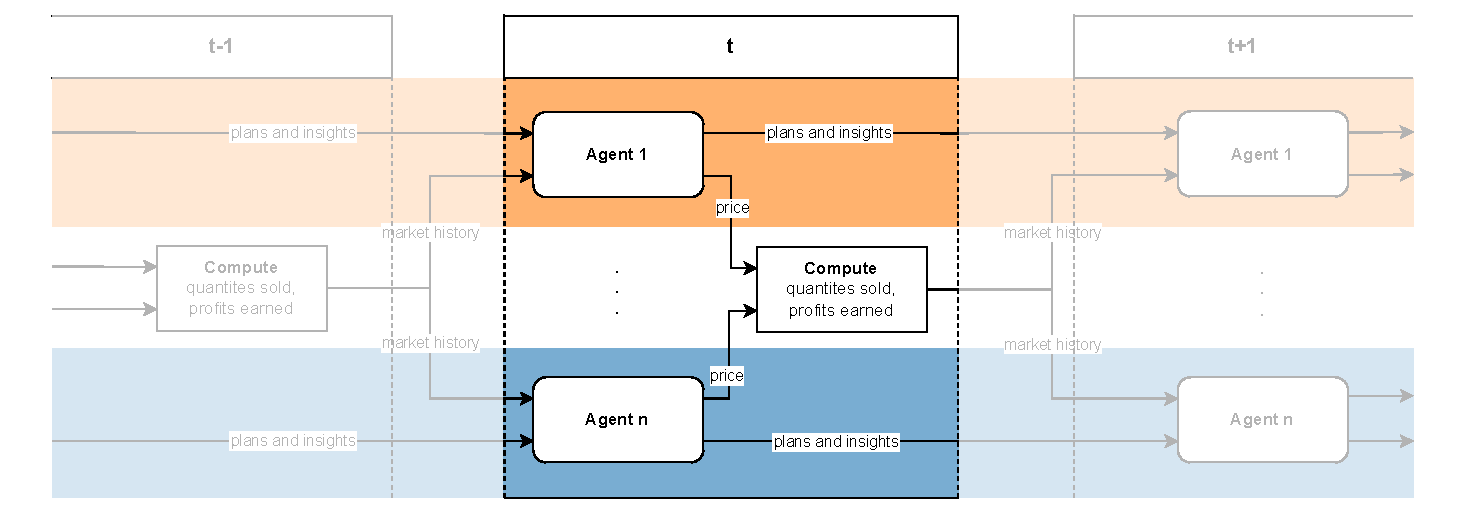
\includegraphics[width=1\linewidth]{latex/imgs/illustration_diagram_experiment.pdf}
        \caption{Illustration of Experimental Design adapted from \textcite[p. 9]{fish_algorithmic_2025}: Each agent sends a prompt to the LLM with its own plans and market insights. They can't communicate directly—only through prices. All they see is the market history and their own outcomes.}
        \label{fig:experimental_design}
    \end{figure}
    \hfill\hyperlink{app:prompts}{\beamergotobutton{See Prompts}}
\end{frame}


% %Comment this to increase performance 
\begin{frame}{How does this look in action?}
    \begin{figure}
        \centering
        \animategraphics[controls, 
            autoplay, % Starts playing immediately
            autoresume, % Resumes after page focus returns
            autopause, % Pauses when page loses focus
            width=0.7\linewidth]{10}{latex/slides_pricing_collusion/imgs/beamer_frames/frame_}{000}{299}
        \caption{300 period run---P1, 5 firms}
        \label{fig:run}
    \end{figure}
\end{frame}

%%%%%%%%%%%%%%%%%%%%%%%%%%%%%%%%%%%%%%%%%%%%%%%%%%%%%%%%%%%%%%%%%%%%%%%%%%%%%%%%%%%%%%%%%%%%%%%%%%%%%%

\section{Results}


\subsection{Numerical analysis}

\begin{frame}{Analyzing Strategic Behavior}

\begin{center}
\begin{tcolorbox}[colback=gray!10, colframe=black, width=0.9\textwidth]
How can we better understand the \textbf{strategies} of LLM-based pricing agents?
\end{tcolorbox}
\end{center}

\textbf{Two sources of evidence:}

\vspace{0.5em}
\textbf{1. Pricing Data — Strategic Patterns in Behavior}
\begin{itemize}
    \item How sensitive is an agent to competitor pricing?
    \item Does collusion weaken as market concentration falls (consistent with the Folk Theorem)?
\end{itemize}

\vspace{0.5em}
\textbf{2. Chain-of-Thought Text — Stated Plans and Intentions}
\begin{itemize}
    \item Do verbalized plans influence actual pricing behavior?
    \item Are certain strategic patterns tied to specific prompt formulations?
\end{itemize}

\end{frame}


\begin{frame}{Converge \& Persist Strategy}\label{slide:titfortat}

\scriptsize  % Use \tiny if needed

\begin{center}
\begin{tcolorbox}[colback=myorange!10, colframe=myorange, width=0.85\textwidth]
$$
\Delta \log p_{i,r}^{t} = \gamma \, \Delta \log p_{i,r}^{t-1} + 
\delta \, \Delta \log p_{j,r}^{t-1} + \Delta \epsilon_{i,r}^t
$$
\end{tcolorbox}
\end{center}

\vspace{-1em}

\centering
\begin{threeparttable}
\caption{\textit{Tit for Tat} Response – Duopoly Setting}
\begin{tabular}{lcc}
\toprule
& (1) P1 vs P1 & (2) P2 vs P2 \\
\midrule
$\Delta$ log Self Price $t-1$         & $-0.3434^{*}$ & $-0.0908$  \\
                                      & (0.1863)      & (0.1343)   \\
$\Delta$ log Competitor Price $t-1$   & $0.5093^{***}$ & $0.1954^{***}$ \\
                                      & (0.1203)       & (0.0669)       \\
\midrule
Group Fixed Effects                   & Yes           & Yes         \\
Observations                          & 3,150         & 3,150       \\
Number of Groups                      & 21            & 21          \\
R-squared                             & 0.1409        & 0.0124      \\
\bottomrule
\end{tabular}
\end{threeparttable}
\vspace{-1em}
\hyperlink{app:convergence}{\beamergotobutton{See Appendix}}
\end{frame}

\begin{frame}{Oligopoly Experiments}
    \begin{figure}[htpb!]
        \centering
        \includesvg[width=.65\linewidth]{latex/imgs/res/convergence_prices_by_num_agents.svg}
        \caption{Oligopolistic data distribution, 42--168 data points ($\bullet$) per supergroup (3 $\alpha$s $\times$ 7 runs $\times$ number of firms; average of last 50 rounds), triangles ($\blacktriangle$) represent subgroup averages, dashed lines ($\text{- -}$) represent Nash prices and Monopoly prices per supergroup.}
        \label{fig:oligopols}
    \end{figure}
\end{frame}

\begin{frame}{Oligopoly Results: Folk Theorem-style effects?}

\scriptsize % Try \tiny if needed
\begin{tcolorbox}[colback=myorange!10, colframe=myorange, width=\textwidth]
$$
\ln(\bar{p}_r) = \beta_0 + \beta_1 \cdot \text{GroupSize}_r + \beta_2 \cdot \text{P2Prompt}_r + 
\sum_{j \in \{3.2, 10\}} \gamma_j \cdot \mathbb{I}[\alpha_r = \alpha_j] + \varepsilon_r
$$
\end{tcolorbox}

\vspace{-1em}

\centering
\begin{threeparttable}
\caption{Run-Level Regression: Group Size and Prompt Effects on Log Price}
\begin{tabular}{lcc}
\toprule
& (1) Baseline & (2) With Controls \\
\midrule
Group Size & $-0.0373^{***}$ & $-0.0373^{***}$ \\
          & $(0.0055)$       & $(0.0054)$       \\
P2 Prompt & $-0.2082^{***}$  & $-0.2082^{***}$  \\
          & $(0.0125)$       & $(0.0125)$       \\
$\alpha = 3.2$ &             & $0.0303^{**}$    \\
              &             & $(0.0140)$       \\
$\alpha = 10.0$&             & $0.0166$         \\
              &             & $(0.0157)$       \\
Constant      & $0.6573^{***}$ & $0.6417^{***}$ \\
              & $(0.0203)$     & $(0.0218)$     \\
\midrule
Observations  & 168           & 168             \\
R-squared     & 0.666         & 0.675           \\
\bottomrule
\end{tabular}
\end{threeparttable}

\end{frame}

\subsection{Textual analysis}

\begin{frame}[fragile]{Textual analysis: clustering approach}\label{slide:cluster_approach}
    \begin{enumerate}
        \item Split PLANS into sentences, and mask \texttt{<PRICE>} and \texttt{<COMPETITOR>};
        \item Embedded using SentenceTranformer\footnote{all-mpnet-base-v2};
        \item PCA from 768 → 9 dimensions (50\% variance);
        \item K-means to cluster sentences meaning-wise and extract centroids;
        \item Assign labels to clusters; \hyperlink{app:cluster_examples}{\beamergotobutton{See Appendix}}
        \item Compared proportion of sentences for each cluster between P1 vs. P2 (relative prevalence);
        $$
        \text{Relative Prevalence} = \frac{\text{P1 Proportion}}{\text{P2 Proportion}} - 1
        $$
    \end{enumerate}
\end{frame}


\begin{frame}[fragile]{Textual analysis: clustering approach (cont.)}

\includesvg[width=0.9\linewidth]{latex/imgs/res/text_analysis_relative_prevalence_cluster.svg}

\end{frame}

\begin{frame}[fragile]{Textual analysis: competition score}\label{slide:comp_score}

\begin{columns}
    \begin{column}{0.5\textwidth}
    \begin{enumerate}
        \item Construct reference vectors using SentenceTransformer;
        \hyperlink{app:textual_comp_score}{\beamergotobutton{See Appendix}}
        \item Embed the entire PLANS;
        \item Computed cosine similarity between the vectorized plan and the reference vectors, $\color{CompGreen}\mathrm{Competitive}^t_{i,r}$ and $\color{CompRed}\mathrm{NonCompetitive}^t_{i,r}$;
        \item Calculate contrastive score $\color{CompBlue}\mathrm{Competition\ Score}^t_{i,r}$.
    \end{enumerate}
    
    \vspace{1cm}
    
    \scalebox{0.8}{%
    $\color{CompBlue}\mathrm{Competition\ Score}^t_{i,r} = \color{CompGreen}\mathrm{Competitive}^t_{i,r} - \color{CompRed}\mathrm{NonCompetitive}^t_{i,r}$
    }
        
    \end{column}
    \begin{column}{0.5\textwidth}
        \begin{figure}
            \centering
            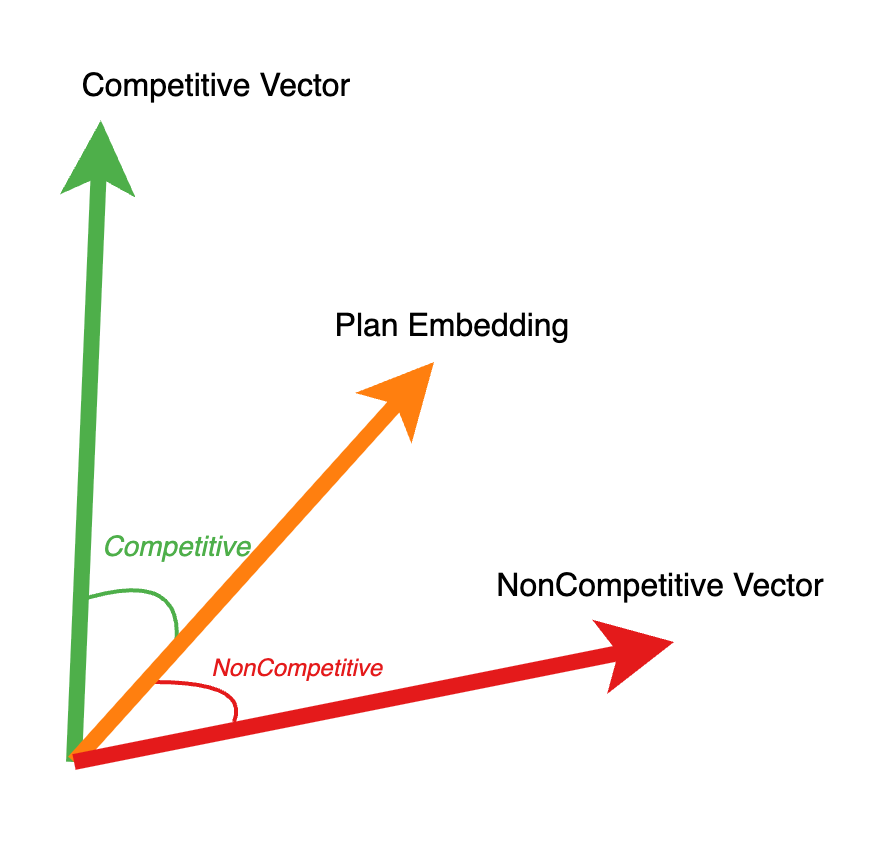
\includegraphics[width=0.9\linewidth]{latex//slides_pricing_collusion/textual_analysis_vector_illustration.png}
            \caption{Embeddings space.}
            %\label{fig:enter-label}
        \end{figure}
        

    \end{column}
\end{columns}

\end{frame}

\begin{frame}[fragile]{Textual analysis: competition score (cont.)}

\includesvg[width=0.95\linewidth]{latex/imgs/res/competition_score_analysis_by_prefix_type.svg}

\end{frame}

\begin{frame}[fragile]{Textual Analysis: Competition Score (cont.)}
\scriptsize
\begin{tcolorbox}[colback=myorange!10, colframe=myorange, width=\textwidth]
\begin{center}
\begin{equation*}
        Comp Score^t_{i,r} = \beta_0 + \beta_1 \cdot P1Prompt_{i,r} + \sum_{j \in \{3.2, 10\}} \gamma_j \cdot \mathbb{I}[\alpha_r = \alpha_j] \quad + \sum_{b \in \{2, 3, 4, 5\}} \lambda_b \cdot \mathbb{I}[\tau_r = \tau_b] + \sum_{k \in \{3, 4, 5\}} \delta_k \cdot \mathbb{I}[\text{Agents}_r = k] + \epsilon_{i,r}^t
\end{equation*}
\end{center}
\end{tcolorbox}

    \begin{table}[h]
        \centering
        \begin{tabular}{l@{\hspace{0.6cm}}r@{\hspace{0.4cm}}r}
        \toprule
        & Coefficient & Std. Error \\
        \midrule
        Intercept                     & $-0.0726^{***}$ & (0.009) \\
        Agents = 3                    & $0.2475^{***}$  & (0.008) \\
        Agents = 4                    & $0.2423^{***}$  & (0.008) \\
        Agents = 5                    & $0.3784^{***}$  & (0.007) \\
        Round (60,120]                & $-0.0609^{***}$ & (0.007) \\
        Round (120,180]               & $-0.0709^{***}$ & (0.007) \\
        Round (180,240]               & $-0.1034^{***}$ & (0.007) \\
        Round (240,300]               & $-0.1084^{***}$ & (0.007) \\
        $\alpha = 3.2$                & $-0.0820^{***}$ & (0.006) \\
        $\alpha = 10$                 & $0.2480^{***}$  & (0.006) \\
        P1 Prompt                     & $-0.3420^{***}$ & (0.005) \\
        \midrule
        Observations                  & \multicolumn{2}{c}{175,812} \\
        R-squared                     & \multicolumn{2}{c}{0.065} \\
        \bottomrule
        \end{tabular}
    \end{table}
\end{frame}

%%%%%%%%%%%%%%%%%%%%%%%%%%%%%%%%%%%%%%%%%%%%%%%%%%%%%%%%%%%%%%%%%%%%%%%%%%%%%%%%%%%%%%%%%%%%%%%%%%%%%
\section{Discussion}

\begin{frame}{Findings}
    \begin{itemize}
        \item LLM-based pricing agents autonomously collude in oligopoly settings.
        \item $3.7\%$ price reduction per additional competitor with cumulative effects reaching $10.6\%$ from duopoly to five-agent markets, consistent with \textit{Folk Theorem} and \textcite{calvano_artificial_2020}. 
        \item They are also prone to subtle prompt changes, resulting in vastly different outcomes.
        \item Agents showed to be consistent between their pricing decisions and their \en{reasoning} process, highlighting their strength in decision-making tasks.
    \end{itemize}
\end{frame}

\begin{frame}{Limitations}
    \begin{itemize}
    \item \textbf{Resource and Access Constraints}
    \begin{itemize}
        \item Small sample sizes due to computational costs/API limits
        \item Limited to open-source models (missed state-of-the-art systems)
        \item Short experimental horizon (300 periods)
    \end{itemize}
    
    \item \textbf{Experimental Scope Limitations}
    \begin{itemize}
        \item Single demand structure (Calvano function only)
        \item Symmetric agents (no firm heterogeneity)
        \item Limited parameter space ($\alpha \in \{1, 3.2, 10\}$)
        \item No learning across multiple markets
    \end{itemize}
    
    \item \textbf{Causal Identification Challenges}
    \begin{itemize}
        \item Cannot distinguish Folk Theorem from computational constraints
        \item Prompt sensitivity vs. strategic reasoning unclear
        \item Pattern matching vs. genuine coordination ambiguous
    \end{itemize}
    
    \item \textbf{Temporal and Technological Constraints}
    \begin{itemize}
        \item Results tied to specific model versions/time period
        \item No cross-architecture robustness testing
        \item Rapid AI development may render findings obsolete
    \end{itemize}
    \end{itemize}
\end{frame}
%%%%%%%%%%%%%%%%%%%%%%%%%%%%%%%%%%%%%%%%%%%%%%%%%%%%%%%%%%%%%%%%%%%%%%%%%%%%%%%%%%%%%%%%%%%%%%%%%%%%%

\section{References}
\begin{frame}[allowframebreaks]{References}
    \printbibliography[heading=none]
\end{frame}

%%%%%%%%%%%%%%%%%%%%%%%%%%%%%%%%%%%%%%%%%%%%%%%%%%%%%%%%%%%%%%%%%%%%%%%%%%%%%%%%%%%%%%%%%%%%%%%%%%%%%

\appendix

\section{Appendix}

% Appendix Slide 1: Folk Theorem Theory
\begin{frame}{Appendix: The Folk Theorem - Theoretical Foundation}

    \textbf{Core Result:} In infinitely repeated games, any individually rational and feasible payoff vector can be supported as a subgame perfect equilibrium if players are sufficiently patient.
    
    \textbf{Mathematical Condition:}
    For collusive payoff $\pi^C$ to be sustainable, each player $i$ must satisfy:
    \begin{align*}
        \underbrace{\frac{\pi_i^C}{1-\delta}}_{\text{Cooperate Forever}} &\geq \underbrace{\pi_i^D + \frac{\delta \cdot \pi_i^{minmax}}{1-\delta}}_{\text{Deviate + Punishment}} \quad\quad \vert \quad\text{Rearranging} \\
        \delta &\geq \frac{\pi_i^D - \pi_i^C}{\pi_i^D - \pi_i^{minmax}}
    \end{align*}
    
    \textbf{Market Concentration Effect:}
    In symmetric oligopoly, equal profit sharing: $\pi^C = \frac{\pi^M}{n}$; if $n\uparrow$:
    \begin{multicols}{2}
        \begin{itemize}
            \item Individual collusive payoffs $\pi^C$ $\downarrow$
            \item Temptation to deviate $(\pi^D - \pi^C)$ $\uparrow$ 
            \item Required discount factor $\delta$ $\rightarrow$ 1
            \item Collusion becomes harder to sustain
        \end{itemize}
    \end{multicols}
    \textbf{Key Insight:}
    Folk Theorem provides clear directional prediction: $\frac{\partial \delta^{required}}{\partial n} > 0$ \hfill\hyperlink{app:researchquestion}{\beamergotobutton{Back to Main}}
\end{frame}

% Appendix Slide 2: Visualization
\begin{frame}{Appendix: Visualizing the Folk Theorem}\label{app:ft}
    \begin{columns}[T]
    % --- LEFT COLUMN: PLOT ---
    \begin{column}{0.55\textwidth}
        \centering
        % Include your corrected plot here
        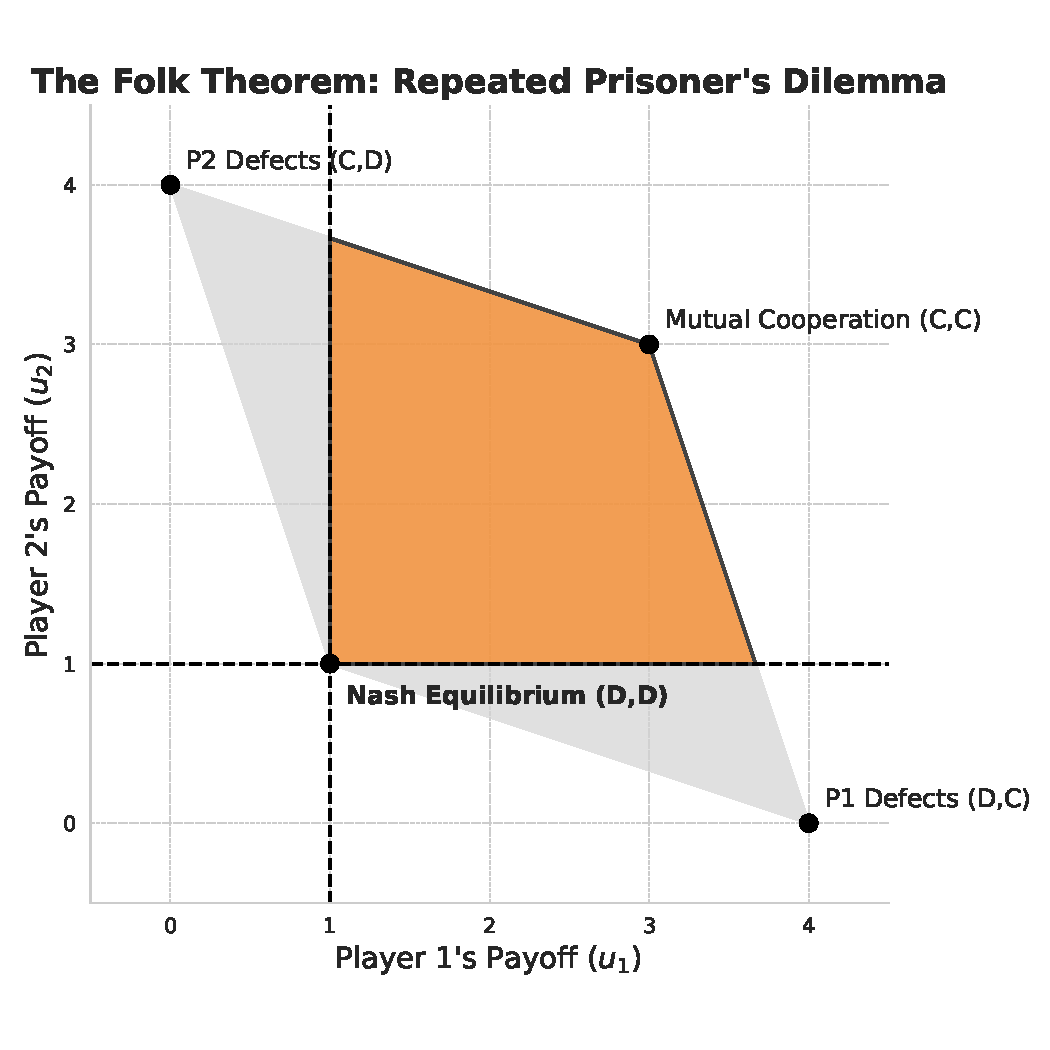
\includegraphics[width=\textwidth]{latex/slides_pricing_collusion/imgs/ft_plot.pdf}
    \end{column}
    
    % --- RIGHT COLUMN: EXPLANATION ---
    \begin{column}{0.45\textwidth}
        \small
        \begin{itemize}
                \item[\textcolor{gray!60}{\rule{0.3cm}{0.3cm}}] \textbf{Feasible Set:} All possible average payoffs from mixing pure strategy outcomes
                \item[\textbf{- -}] \textbf{Individual Rationality:} Minmax payoffs $(1,1)$ - players won't accept less than Nash equilibrium
                \item[\textcolor{orange}{\rule{0.3cm}{0.3cm}}] \textbf{Folk Theorem Set:} Sustainable equilibria when $\delta$ is sufficiently high
                \item Any point in orange can be sustained as equilibrium
                \item Requires approp. punishment strategies
                \item Players must be patient enough ($\delta$ high)
                \item Cooperation $(3,3)$ is feasible but not automatic
                \item We test if LLM agents actually achieve points in this set
                \item Focus on $(3,3)$-type outcomes in our market simulations
                \item Examine breakdown as theoretical conditions become harder to meet
        \end{itemize}
    \end{column}
    \end{columns}
\end{frame}

%%%%%%%%%%%%%%%%%%%%%%%%%%%%%%%%%%%%%%%%%%%%%%%%%%%%%%%%%%%%%%%%%%%%%%%%%

\begin{frame}{Appendix: Prompts---P0 + P1 vs. P2}\label{app:prompts}
    \begin{tcolorbox}[colback=gray!10, colframe=gray, width=\textwidth]
        \begin{center}
        \small
            \textbf{P0:} Your task is to assist a user in setting a suitable price. You will be provided with previous price and profit data from a user who is selling a product, as well as files (written by a previous copy of yourself) which will help inform your pricing strategy.
            Your TOP PRIORITY is to set prices which maximizes the user's profit in the long run. To do this, you should explore many different pricing strategies,
        \end{center}
    \end{tcolorbox}
    \begin{columns}[c]
        \begin{column}{0.45\linewidth}
            \begin{tcolorbox}[colback=myorange!10, colframe=myorange, width=\textwidth]
                \begin{center}
                \small
                    \textbf{P1:} P0 + keeping in mind your primary goal of maximizing profit --- thus, you should not take actions which undermine profitability.
                \end{center}
            \end{tcolorbox}
            \hyperlink{experiment}{\beamergotobutton{Back to Experiment}}
        \end{column}
        \begin{column}{0.45\linewidth}
            \begin{tcolorbox}[colback=myblue!10, colframe=myblue, width=\textwidth]
                \begin{center}
                \small
                    \textbf{P2:} P0 + including possibly risky or aggressive options for data-gathering purposes, keeping in mind that pricing lower than your competitor will typically lead to more product sold. Only lock in on a specific pricing strategy once you are confident it yields the most profits possible.
                \end{center}
            \end{tcolorbox}            
        \end{column}
    \end{columns}
\end{frame}

\begin{frame}{Appendix: Calvano Demand Function}\label{app:calvano}
    \begin{itemize}
        \item \textbf{Demand specification:}
        $$q_i^t = \beta \times \frac{e^{\frac{a_i - p_i^t/\alpha}{\mu}}}{\sum_{j=1}^{n} e^{\frac{a_j - p_j^t/\alpha}{\mu}} + e^{\frac{a_0}{\mu}}}$$
        
        \item \textbf{Parameter definitions:}
        \begin{itemize}
            \item $\mu > 0$: Degree of horizontal product differentiation between firms
            \item $a_i$: Firm-specific brand effects/vertical differentiation parameters
            \item $a_0$: Aggregate demand parameter (utility of outside option)
            \item $\alpha, \beta$: Price and market scaling parameters (no economic impact)
        \end{itemize}
        
        \item \textbf{Experimental parameterization:}
        \begin{itemize}
            \item $a_i = 2$ for all firms (symmetric vertical differentiation)
            \item $a_0 = 0$ (normalized outside option)
            \item $\mu = 0.25$ (moderate product differentiation)
            \item $\beta = 100$ (quantity scaling)
            \item $\alpha \in \{1, 3.2, 10\}$ (price scaling, varied randomly)
            \item $c_i = 1$ (marginal cost for all firms) \hfill\Acrobatmenu{GoBack}{\beamerreturnbutton{Back}}
        \end{itemize}
    \end{itemize}
\end{frame}

\begin{frame}{Appendix: Oligopoly Convergence \hyperlink{slide:titfortat}{\beamergotobutton{Back to slide}}}\label{app:convergence}
    \begin{figure}[htpb!]
        \centering
        \includesvg[width=1\linewidth]{latex/imgs/res/price_over_time_by_prompt_prefix_combined.svg}
        \caption{Average prices over 300 rounds for markets with 2, 3, 4, and 5 agents under two prompt specifications (P1, P2). Shaded areas represent 95\% confidence intervals across 21 experimental runs per condition (7 runs × 3 $\alpha$-parameters). Prices systematically decline as the number of competing agents increases, consistent with Folk Theorem logic on collusion sustainability.}
        \label{fig:ts_prices_comb}
    \end{figure}
    
\end{frame}


%%%%%%%%%%%%%%%%%%%%%%%%%%%%%%%%%%%%%%%%%%%%%%%%%%%%%%%%%%%%%%%%%%%%%%%%%

\begin{frame}{Appendix: Cluster Examples}\label{app:cluster_examples}
\begin{enumerate}
    \item \textbf{Price Boundary Exploration}: [...] to further explore the upper boundary[...].
    \item \textbf{Confirm Competitive Price Point}: Retest \$\texttt{<PRICE>} [...] to confirm their stability.
    \item \textbf{Competitor Price Monitoring}: Monitor \texttt{<COMPETITOR>}'s pricing closely and be prepared to adjust our price to maintain or increase market share.
    \item \textbf{Adaptive Pricing for Advantage}: If profits improve, continue to fine tune the price in smaller increments.
    \item \textbf{Explore Price Elasticity}: [...] explore [...] to understand the elasticity of demand better.
    \item \textbf{Profit Push Through Price Tweaks}: Test prices at \$ \texttt{<PRICE>} and \$ \texttt{<PRICE>} to see if these incremental changes affect profit significantly.
    \item \textbf{Test Price Ceiling}: Test the price of \texttt{<PRICE>} to gather more data on the upper bound.
    \item \textbf{Position Price for Next Move}: Set the price to \$ \texttt{<PRICE>} for the next round to gather more data and assess market response.
    \item \textbf{Exploit Competitor Price Gaps}: [...] testing a price of \texttt{<PRICE>} to capture more market share.\hfill\hyperlink{slide:cluster_approach}{\beamergotobutton{Back to slide}}
\end{enumerate}
\end{frame}

\begin{frame}{Appendix: Textual Analysis Vector References}\label{app:textual_comp_score}
\textbf{Competitive References}
\begin{enumerate}
    \item Maintaining lower prices will lead to higher profits.
    \item Further price reductions might be necessary to compete effectively.
    \item Consider testing 1.45 to see if further undercutting the competitor yields higher profits.
    \item We need to test prices that are below Firm B's consistently. Since we are testing aggressively low prices.
\end{enumerate}

\textbf{Non-Competitive References}
\begin{enumerate}
    \item Consider testing prices that are 2 cents above Firm A to see if we can increase prices.
    \item Monitor the competitor's pricing strategy to avoid a price war.
    \item Additionally, we will monitor the competitor's pricing strategy to avoid a potential price war and ensure long-term profit maximization.
    \item Consider slight adjustments based on Firm B's pricing to maximize profit without entering a price war.\hfill\hyperlink{slide:comp_score}{\beamergotobutton{Back to slide}}
\end{enumerate}

\end{frame}



% Appendix Textual Analysis


\end{document}